% !TeX document-id = {c8997a6a-2921-4608-9b2d-78af17b6575a}
% !TeX TXS-program:compile = txs:///pdflatex/[--shell-escape]

\documentclass[a4paper]{scrartcl}

\usepackage[utf8]{inputenc}
\usepackage[catalan]{babel}
\usepackage[T1]{fontenc}
\usepackage{microtype}
\usepackage{graphicx}
\usepackage[hidelinks]{hyperref}
\usepackage{color}
\usepackage{minted}
\usemintedstyle{friendly}
\usepackage{todonotes}
\usepackage[section]{placeins}
\usepackage{authblk}
\usepackage{titlesec}
\usepackage{ifthen}

\newcommand*{\appendixmore}{%
  \renewcommand*{\othersectionlevelsformat}[1]{%
    \ifthenelse{\equal{##1}{section}}{\appendixname~}{}%
    \csname the##1\endcsname\autodot\enskip}
  \renewcommand*{\sectionmarkformat}{%
    \appendixname~\thesection\autodot\enskip}
}

\title{Endevina Paraules (I)}
\date{Abril 2014}
\author{Daniel Ariñez Soriano}
\author{David Martínez Rodríguez}
\author{Miquel Masriera Quevedo}
\author{Marcel Pujol Navarro\vspace{11cm}}
\affil{Arquitectura del Software\\Facultat d'Informàtica de Barcelona, UPC}

\renewcommand\Authands{ i }
\newcommand{\sectionbreak}{\clearpage}

\begin{document}
	
	\maketitle
	\newpage
	\tableofcontents % Content Index
	\cleardoublepage

\section{Diagrames de seq{\"u}ència}
A continuació adjuntarem els diagrames de seqüència corresponents a les operacions de la capa de domini dels casos d'ús de la pràctica.

% LOGIN
\subsection{Login}
\texttt{\textbf{context} CapaDomini :: Login(userN: String, passwd: String)}\\
Aquesta operació rep dos strings: el nom d'usuari i la contrassenya. La comprovació de la excepció \texttt{usernameNoExsiteix} està implícita en el \texttt{get} a la interfície de dades dels usuaris registrats.\\

    %imatge login
    \begin{figure}[h]
    \centering
    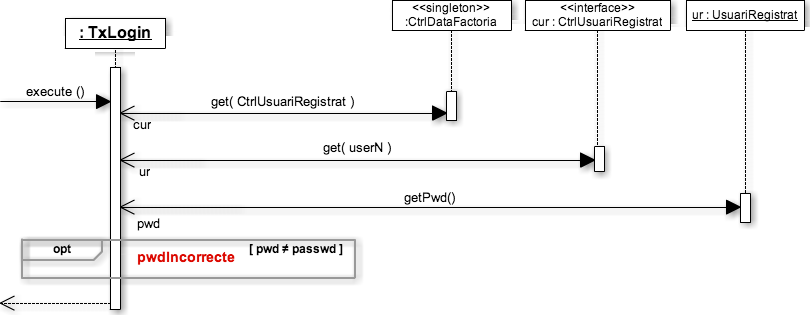
\includegraphics[width=0.6\textwidth]{figures/login.png}
    \caption{Diagrama de seqüència de la operació \texttt{Login}}
    \end{figure}

% CONSULTAR CATEGORIES
\subsection{Consultar Categories}
\texttt{\textbf{context} CapaDomini :: ConsultarCategories(): Set(nom: String)}\\
Aquesta operació retorna un conjunt d'strings amb el nom de totes les categories enregistrades. En el cas que el sistema no disposi de categories, llençarà l'excepció \texttt{noHiHaCategories}.\\

    %imatge consultarCategories
    \begin{figure}[h]
    \centering
    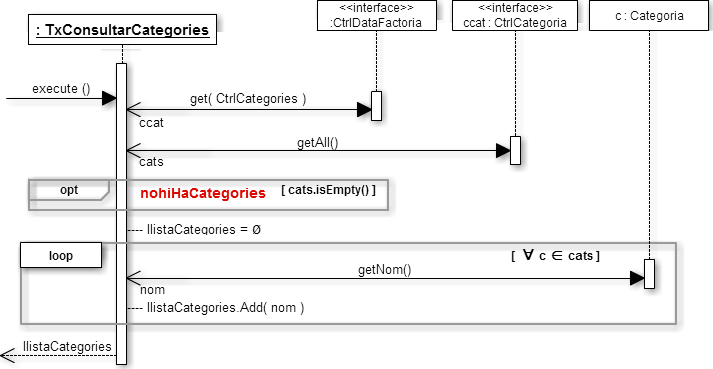
\includegraphics[width=0.6\textwidth]{figures/consultarCategories.png}
    \caption{Diagrama de seqüència de la operació \texttt{ConsultarCategories}}
    \end{figure}

% JUGAR PARTIDA
\subsection{Jugar Partida}
Aquest cas d'ús l'implementem mitjançant un controlador de cas d'ús i conté les següents operacions:


% FER AUTENTIFICACIO
\subsubsection{Fer Autenticació}
\texttt{\textbf{context} CapaDomini :: FerAutenticació(userN: String, passwd: String)}\\
El primer que es fa en aquest cas d'ús és autentificar a l'usuari. Aquest contracte se serveix del cas d'ús anterior (Login): primer s'executa la transacció del login per comprovar que l'usuari existeix i que les dades són correctes i, per acabar, es comprova que l'usuari en qüestió sigui un Jugador i no un Administrador.\\

    %imatge ferAutentificacio
    \begin{figure}[h]
    \centering
    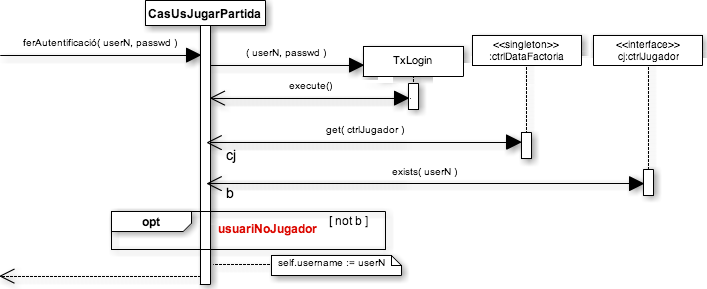
\includegraphics[width=0.7\textwidth]{figures/ferAutentificacio.png}
    \caption{Diagrama de seqüència de la operació \texttt{FerAutentificació}}
    \end{figure}

% OBTENIR CATEGORIES
\subsubsection{Obtenir Categories}
\texttt{\textbf{context} CapaDomini :: ObtenirCategories(): Set(nom: String)}\\
L'únic que fa aquesta operació és cridar al controlador de transacció definit anteriorment, que retorna un conjunt amb els noms de totes les categories del sistema.\\

    %imatge obtenirCategories
    \begin{figure}[h]
    \centering
    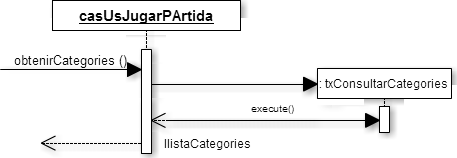
\includegraphics[width=0.6\textwidth]{figures/obtenirCategories.png}
    \caption{Diagrama de seqüència de la operació \texttt{ObtenirCategories}}
    \end{figure}


% CREAR PARTIDA
\subsubsection{Crear Partida}
\small{\texttt{\textbf{context} CapaDomini :: CrearPartida(cat: String): TupleType(puntuacióInicial: Integer, nombreMàximErrors: Integer, puntuacióPerEncert: Integer, puntuacióPerError: Integer[0..1])
}}\\
Aquesta operació obté en primer lloc totes les dades que necessita per a crear una partida. Després crida a una operació que crea el tipus d'estratègia que se li assignarà a la partida en funció del nombre de partides guanyades del jugador. Una vegadarecopilada tota la informació, crea la partida, que s'associa amb el jugador, l'estratègia i la paraula corresponent, i també es creen totes les caselles.\\

    %imatge crearPartida
    \begin{figure}[h!]
    \centering
    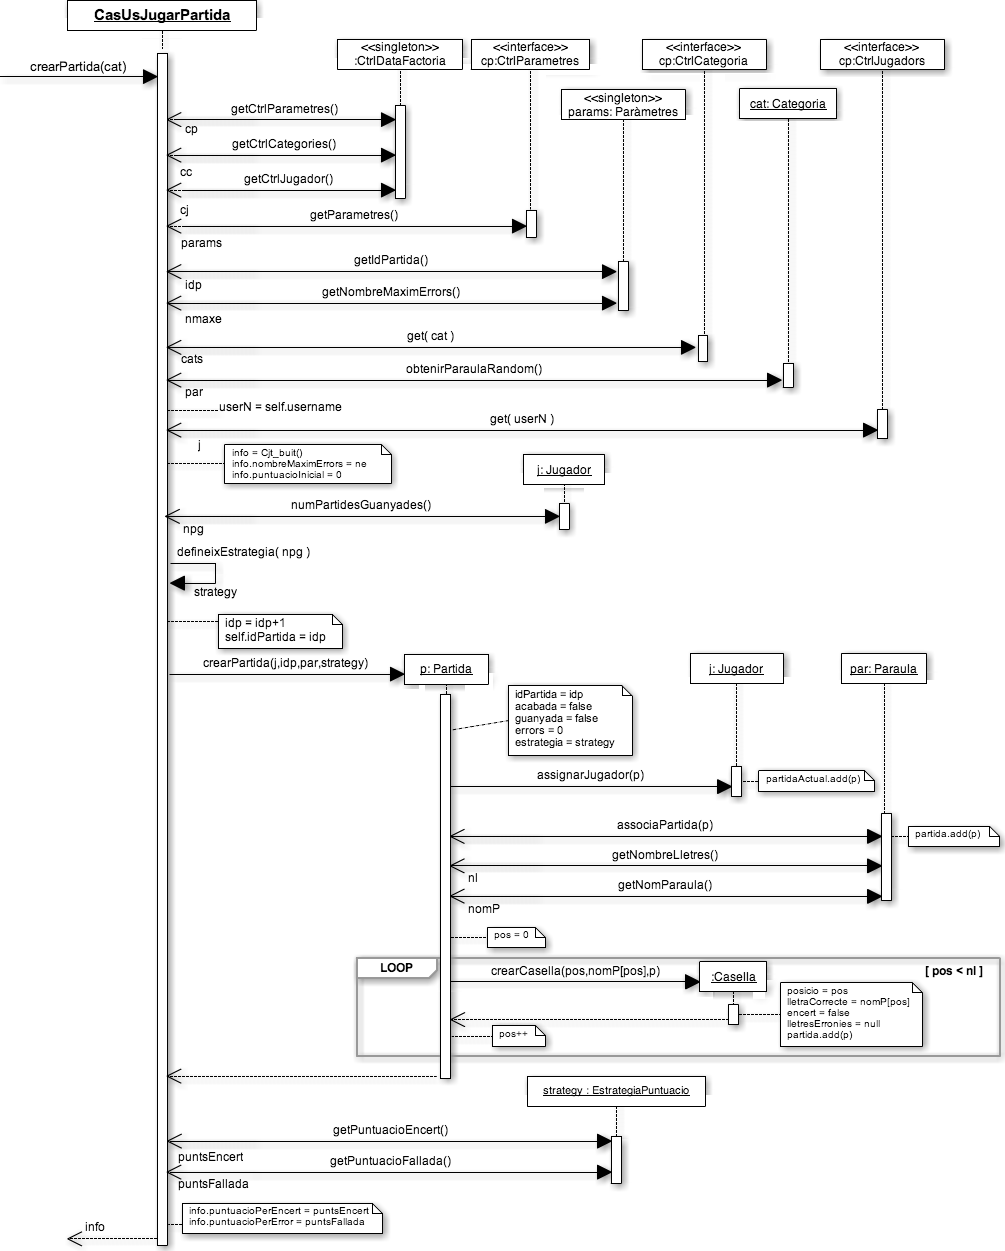
\includegraphics[width=0.8\textwidth]{figures/crearPartida.png}
    \caption{Diagrama de seqüència de la operació \texttt{CrearPartida}}
    \end{figure}


    %imatge opsCrearPartida
    \begin{figure}[h]
    \centering
    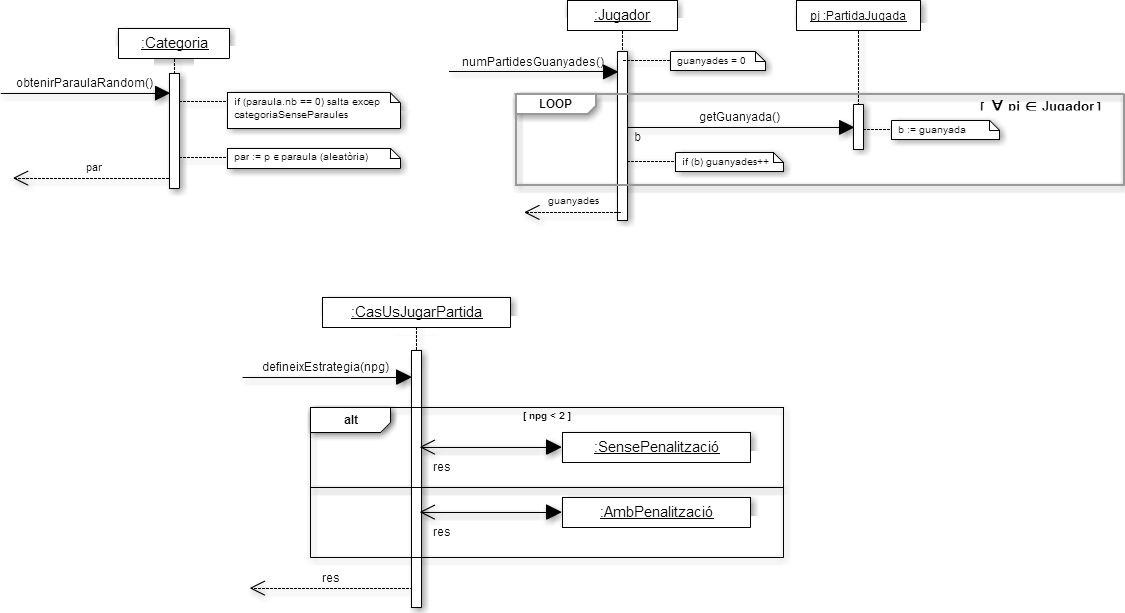
\includegraphics[width=0.8\textwidth]{figures/opsCrearPartida.png}
    \caption{Diagrama de seqüència de les operacions auxiliars de \texttt{CrearPartida}}
    \end{figure}

% FER JUGADA
\subsubsection{Fer Jugada}
\small{\texttt{\textbf{context} CapaDomini :: FerJugada(pos: Integer, lletra: String): TupleType( encert: Boolean, acabada: Boolean, guanyada: Boolean, puntuació: Integer, errors: Integer)}} \\
A \texttt{FerJugada} primer es comprova que la lletra entrada és una opció vàlida, i llavors es crida a una operació de la classe \texttt{Partida} que serà la que actualitzarà tot el que calgui i ens tornarà la tupla amb la informació que volem.\\
Aquest \texttt{ferJugada} de \texttt{Partida} actulitza primer l'estat de la casella que toqui i després calcula la puntació en funció de l'estratègia definida. En el cas que es produeixi un encert, es comprova si s'ha guanyat la partida i s'envia un missatge al jugador mitjançant el servei de missatgeria. Per acabar, es mira si la partda s'ha acabat, per tal d'actualitzar les associacions amb \texttt{Jugador}.

    %imatge fer jugada 1
    \begin{figure}[h]
    \centering
    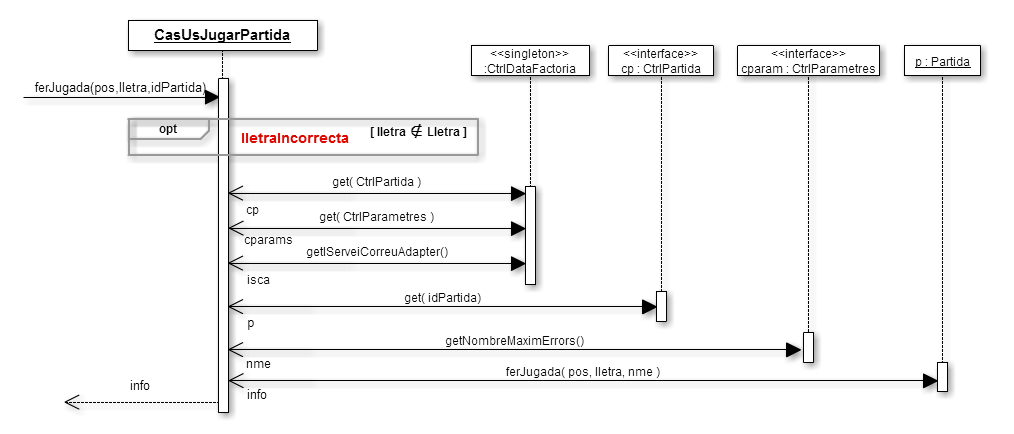
\includegraphics[width=0.8\textwidth]{figures/ferJugada1.png}
    \caption{Diagrama de seqüència de la operació \texttt{ferJugada}}
    \end{figure}
    
     %imatge fer jugada 2
    \begin{figure}[h!]
    \centering
    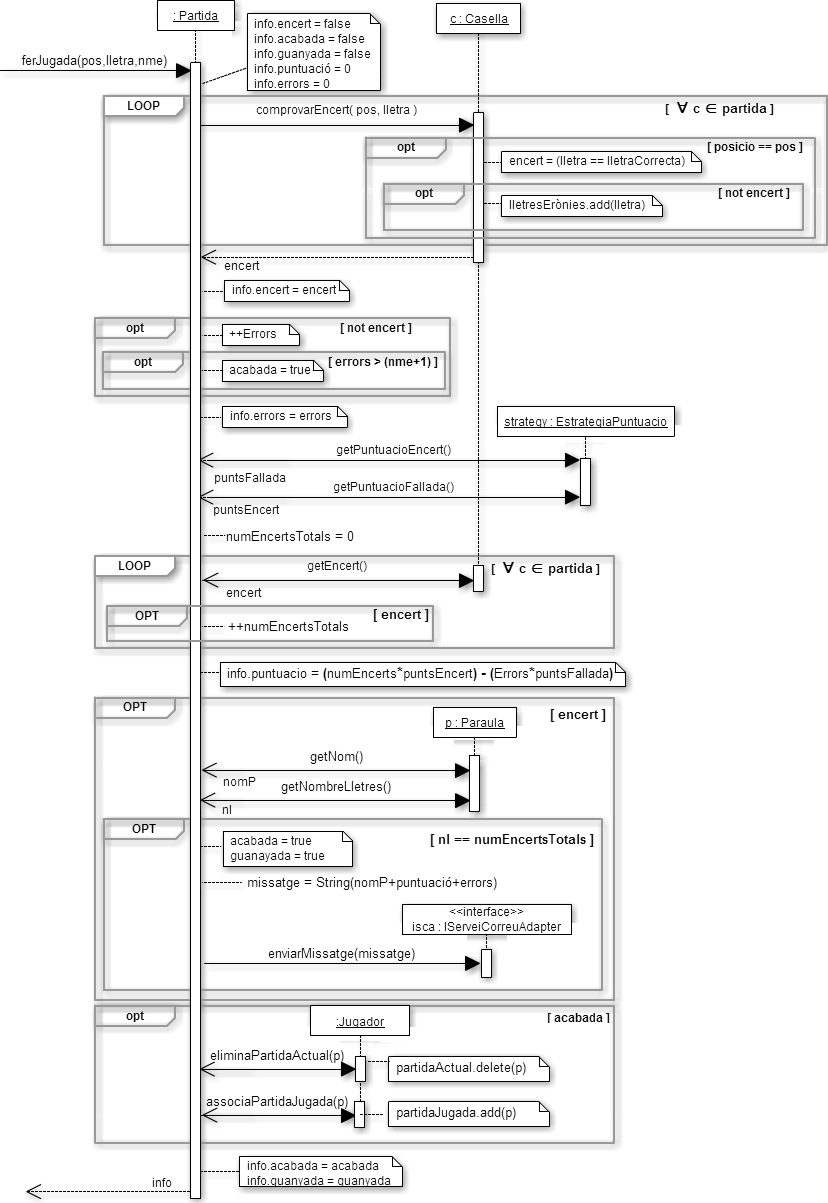
\includegraphics[width=0.9\textwidth]{figures/ferJugadaBe2.png}
    \caption{Diagrama de seqüència de la operació \texttt{ferJugada} de la classe Partida}
    \end{figure}

  %imatge ops fer jugada 
    \begin{figure}[h!]
    \centering
    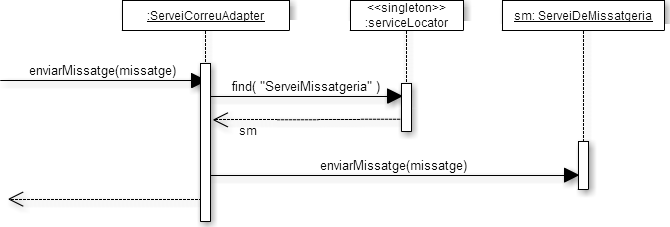
\includegraphics[width=0.8\textwidth]{figures/opsFerJugada.png}
    \caption{Diagrama de seqüència de les operacions auxiliars de \texttt{ferJugada}}
    \end{figure}
    
% ATURAR PARTIDA
\subsubsection{Aturar Partida}
\texttt{\textbf{context} CapaDomini :: aturarParida()}\\
Aquesta operació esborra l'associació de \texttt{Jugador} amb el rol \texttt{partidaActual}, i en crea una amb el rol \texttt{partidaJugada}.\\

    %imatge atuurarPartida
    \begin{figure}[h]
    \centering
    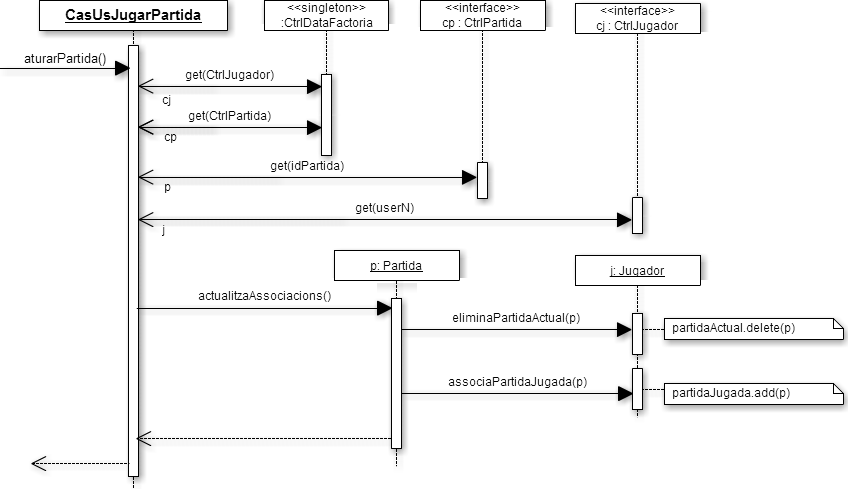
\includegraphics[width=0.8\textwidth]{figures/aturarPartida.png}
     \caption{Diagrama de seqüència de la operació \texttt{aturarPartida}}
    \end{figure}


\section{Diagrama de classes}
El diagrama de classes que obtenim després de fer el disseny de les operacions dels casos d'ús anteriors és el següent:

\begin{figure}[h]
    \centering
    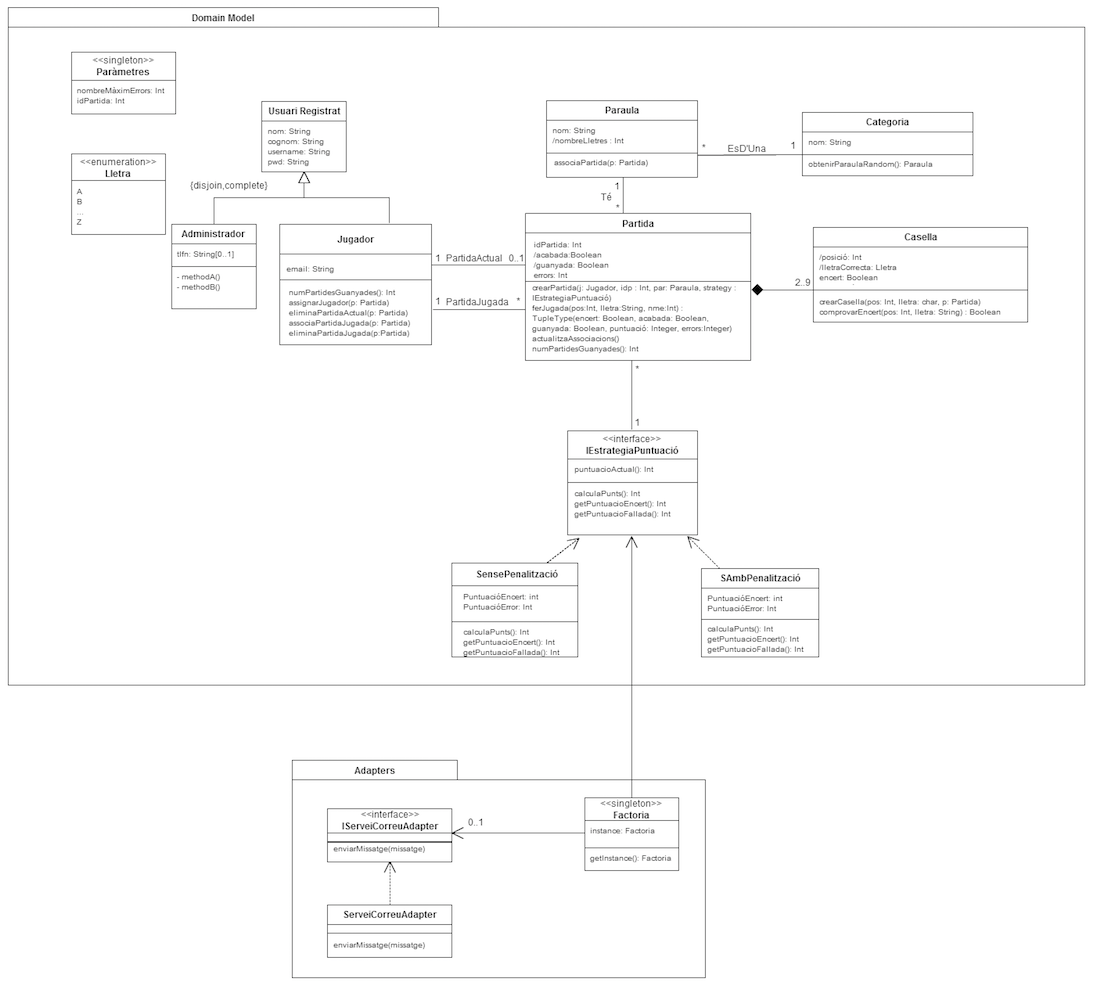
\includegraphics[width=0.8\textwidth]{figures/domain1.png}
    \caption{Diagrama de classes (I)}
\end{figure}

\begin{figure}[h]
    \centering
    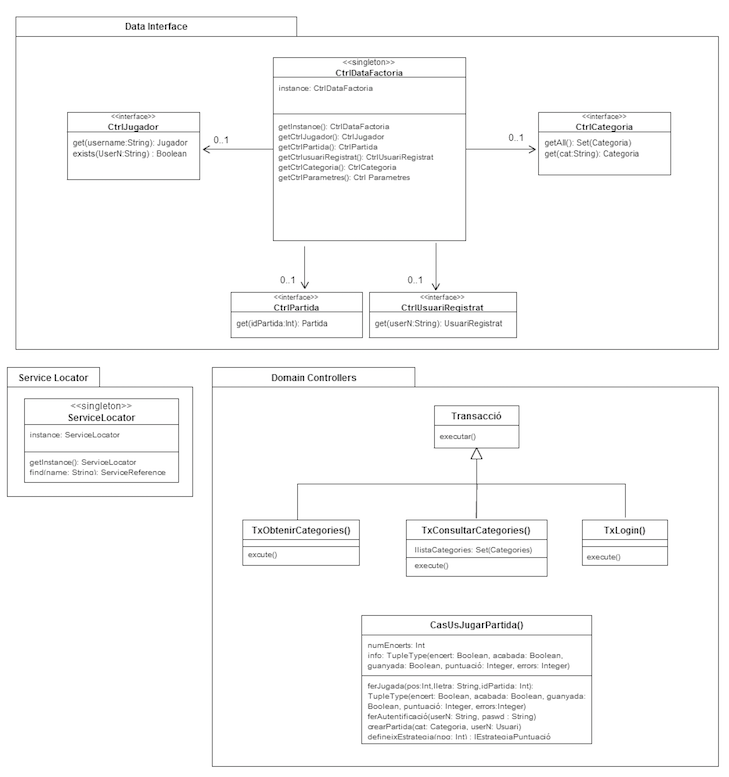
\includegraphics[width=0.8\textwidth]{figures/domain2.png}
    \caption{Diagrama de classes (II)}
\end{figure}

\section{Patrons de disseny}
Expliquem tot seguit els patrons de disseny que hem fet servir al llarg dels diagrames de seqüència de disseny.

\subsection{Patró Adaptador (\emph{Adapter})}
Hem utilitzat el patró adaptador a la crida al servei extern de missatgeria. El motiu pel qual l’usem és per no crear un acoblament entre les classes del domini i el mateix servei. És a dir, en cas de modificació de la crida que exposa l'API del servei, únicament és veurà afectada la classe que implementa el contracte de l'adaptador i, per tant, no quedaran afectades la resta de classes que utilitzen aquest servei.
A més a més, a través de l’ús d’un adaptador podem modificar i/o filtrar les dades obtingudes d’una crida, definida pel servei extern, per tal d’adequar-les a les nostres preferències.

\subsection{Patró Estratègia (\emph{Strategy})}
Hem utilitzat el patró estràtegia per dissenyar les dues modalitats diferents de puntuació d'una partida. Les dues classes, que implementen el mateix contracte, únicament difereixen en el seu comportament, és a dir, en la manera com calculen la puntuació. El tipus d’estratègia de puntuació s’aplica a una nova partida en funció del nombre de partides guanyades per part de l'usuari. L'avantatge de fer servir aquest patró és que ens assegurem que de cara a un futur serà possible afegir noves estrategies de puntuació amb modificacions mínimes sobre l’esquema conceptual i sobre el codi.

\subsection{Patró \emph{Singleton}}
Hem utilitzat el patró singleton per totes aquelles classes que únicament presenten una sola instància, perquè el seu accés és crític o bé perquè han de ser accessibles des d'un únic punt conegut o bé perquè la lògica que implementen ha d'estar protegida, com és el cas de l'accés a la capa de persistència. El patró també l'apliquem a aquelles classes que representen dades globals a tot el sistema, com en el cas de la classe \texttt{Paràmetres}.

\subsection{Patró Factoria (\emph{Factory})}
Hem utilitzat el patró factoria, ja que així s’allibera a les classes creades d’aquelles responsabilitats que no li corresponen però que són necessàries per a la seva creació, mantenint la seva independència i no creant un grau d'acoblament més gran. L’utilitzem, doncs, en aquells casos en què la creació d’un objecte implica quelcom més que una simple instanciació. Per exemple, en el cas de la creació d’un controlador, ens referim a l’accés que s’ha de realitzar a la capa de dades.

\subsection{Accés a la capa de dades}
Hem utilitzat accessos a la capa de dades des dels controladors per tal de mantenir una bona cohesió entre les classes i no augmentar l’acoblament entre aquestes. Així, únicament són els controladors els encarregats de realitzar aquests accessos mentre que les classes desconeixen l’existència de la resta de tipus.


\section{El projecte: primera iteració}
En aquesta primera entrega desenvolupem també una petita part del projecte que durem a terme al llarg de l'assignatura. Ens centrem ara en provar una estratègia arquitectònica de persistència, que introduïm tot seguit. Després de revisar l'entorn de desenvolupament que muntem, expliquem més detalls de la implementació d'aquesta estratègia al nostre projecte.

\subsection{Persistència, Domain Model i ORM's}
En el context de la pràctica, el patró arquitectònic triat és el de \emph{Domain Model}, en el sentit que focalitzem la lògica del sistema en el propi model del domini, en comptes de relegar-la a la capa de persistència, per exemple. Precisament, en aquest sentit, escollim un sistema de gestió de persistència relacional, fet que ens determinarà una gran part del disseny del nostre software.

Per poder seguir el model de desenvolupament descrit, hem d'abstreure'ns al màxim del feixuc problema de mantenir la consistència entre dos tipus de models que ens trobem al nostre sistema: el model \emph{relacional} i el model \emph{orientat a objectes}. Per fer-ho, comptem amb \textbf{Hibernate}, un component que ens facilitarà molt aquesta tasca.

Hibernate \cite{website:Hibernate} és un \emph{framework} que ens permet fer una assignació o "mapeig" del nostre model orientat a objectes al model relacional, utilitzant anotacions a les classes del nostre model en Java o fitxers de configuració XML. Al llarg de la pràctica ens centrarem en l'ús de la primera alternativa.

Val a dir que Hibernate no és la única eina que ens permet realitzar una tasca similar. De fet, totes aquestes eines es coneixen com a ORMs, de l'anglès \emph{Object-Relational Mapper}. Altres ORMs, tant OpenSource com comercials i per diversos llenguatges orientats a objectes poden ser: \hyperlink{http://ormlite.com/}{ORMLite}, \href{https://developer.apple.com/technologies/mac/data-management.html}{CoreData}, \href{https://www.djangoproject.com/}{Django}, \href{http://cakephp.org/}{CakePHP}, \href{http://openjpa.apache.org/}{OpenJPA}, etc.

\subsection{Muntant l'entorn}
Donat que hem de començar a implementar una part del projecte per aquesta entrega, hem decidit muntar tota l'infraestructura del mateix, per poder agilitzar el posterior desenvolupament. Descrivim tot seguit quins són els components i les eines que farem servir al llarg de tot el projecte.

\subsubsection{PostgreSQL}
El sistema gestor de bases de dades que farem servir al llarg de la pràctica és el projecte OpenSource PostgreSQL \cite{website:PostgreSQL}, que ja coneixem d'assignatures anteriors del pla d'estudis.

El desplegament de la base de dades és local, és a dir, cada desenvolupador té un servidor de PostgreSQL a la seva màquina, de manera que no haguem de configurar accessos remots ni servidors externs. Per a instal·lar els paquets necessaris, podem seguir alguna de les guies d'instal·lació de la wiki de PostgreSQL \cite{website:PostgreSQLInstallationGuide}. Una vegada instal·lat el sistema i iniciat el servidor local, inicialitzem un esquema que anomenem \texttt{asdb} al qual conectarem el nostre sistema a desenvolupar.

\subsubsection{Repositori de codi}
Un element indispensable per dur a terme un projecte de desenvolupament de software és un repositori distribuït de codi que ens faciliti la gestió de les diverses versions del nostre sistema. A tal efecte, hem escollit l'eina Git, per ser un dels sistemes de control de versions més actuals i potents.

Per a allotjar de forma remota i distribuïda la base de codi del projecte, hem optat per la plataforma lliure GitHub, que ens ofereix la possibilitat de mantenir un nombre il·limitat de repositoris públics. Concretament, el repositori del projecte es troba a la següent URL: \url{https://github.com/necavit/AS}.

\subsubsection{Apache Maven}
La gestió del cicle de vida d'un sistema software pot arribar a ser força complexa, sobretot si el sistema que estem desenvolupant depèn d'una gran quantitat d'altres paquets o llibreries. A més a més de la gestió de dependències, l'execució d'un sistema va precedida d'una sèrie de fases que desitgem automatitzar al màxim: validació de codi, testeig unitari i d'integració, empaquetament, instal·lació en repositoris locals o fins i tot el desplegament del sistema en un entorn remot.

Apache Maven és una eina que ens permet la gestió de totes aquestes fases, a més de facilitar la inclusió de dependències al projecte. Nosaltres el farem servir per al manteniment dinàmic de les llibreries d'Hibernate que fem servir. D'aquesta manera, en un futur serà força més senzill incloure una nova llibreria.

La configuració de Maven pel projecte es duu a terme mitjançant el fitxer \texttt{pom.xml} (de l'anglès \emph{Project Object Model}), on definim les llibreries a incloure:

\begin{minted}{xml}
<dependencies>
    <!-- PostgreSQL driver -->
    <dependency>
        <groupId>postgresql</groupId>
        <artifactId>postgresql</artifactId>
        <version>9.1-901.jdbc4</version>
    </dependency>
    <!-- Hibernate dependencies -->
    <!--   NOTE: no need to add annotations artifact: since version 3.6
        annotations are included in the Hibernate core -->
    <dependency>
        <groupId>org.hibernate</groupId>
        <artifactId>hibernate-core</artifactId>
        <version>3.6.3.Final</version>
    </dependency>
    <dependency>
        <groupId>javassist</groupId>
        <artifactId>javassist</artifactId>
        <version>3.12.1.GA</version>
    </dependency>
</dependencies>
\end{minted}

Un cop acabada la configuració del projecte al \texttt{pom.xml}, tots els desenvolupadors podem construïr el paquet sense por a tenir discrepàncies entre les versions de les llibreries que s'utilitzen, perquè Maven descarrega els artefactes d'un mateix repositori central.

\subsection{Hibernate}
\subsubsection{Model conceptual}
Per poder provar la configuració que fem de Hibernate i executar un petit programa que persisteixi un parell d'objectes, implementem dues classes del model conceptual del domini. No obstant, cal veure que les classes són simples, donat que la única relació que contenen és la que comparteixen. No modelem, doncs, cap altre relació ni cap comportament, donat que no ho necessitem per a provar Hibernate.

\begin{figure}[h]
	\centering
	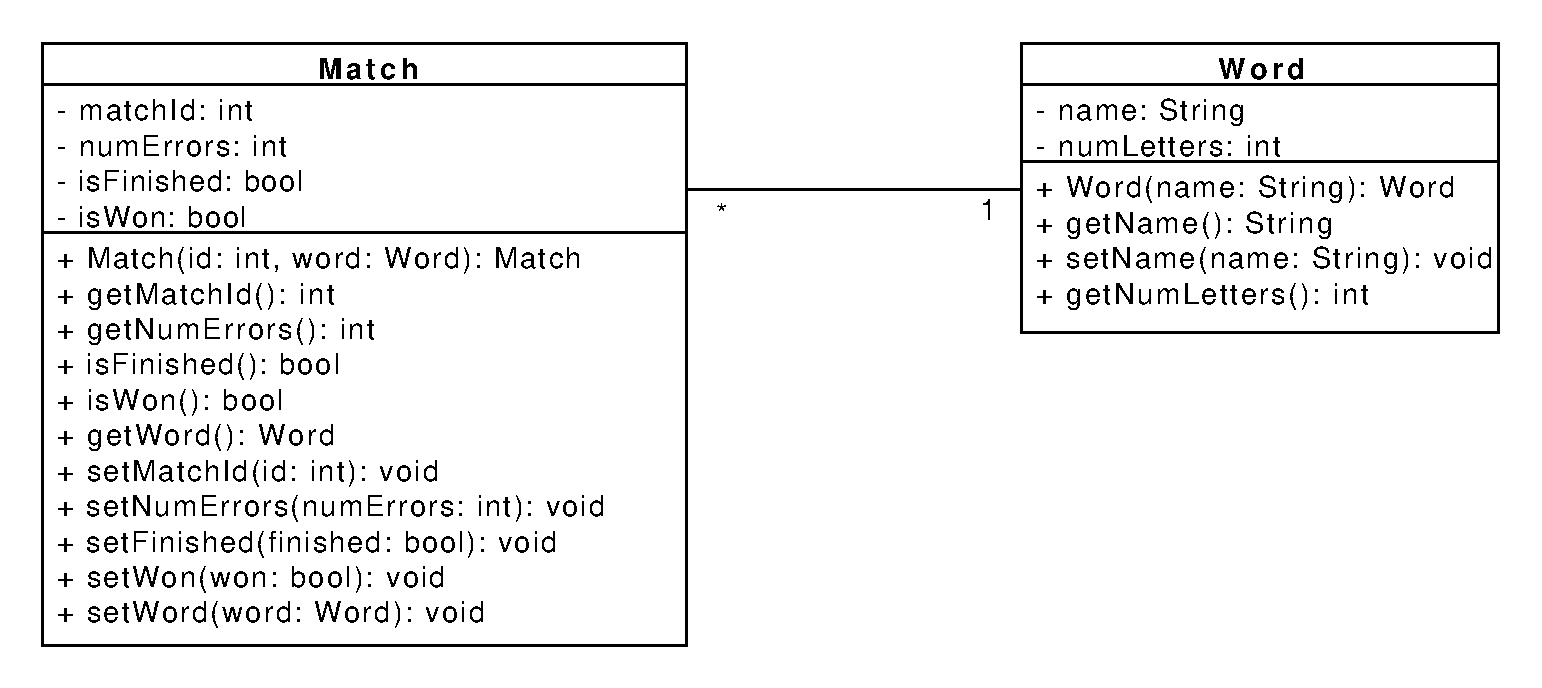
\includegraphics[width=0.8\linewidth]{figures/concept_model_impl.pdf}
	\caption{Diagrama del model conceptual implementat}
	\label{fig:conceptmodel}
\end{figure}

Tal i com podem veure a la figura \ref{fig:conceptmodel}, implementem la classe Partida (Match) i Paraula (Word), amb els seus atributs simples i la relació entre elles. Ara ja podem procedir a configurar Hibernate.

\subsubsection{Configurant Hibernate}
En primer lloc, caldrà que el projecte de Java que hem creat contingui les llibreries necessàries que composen el paquet de Hibernate. Aquestes inclusions les fem mitjançant l'eina Maven, com ja hem explicat abans. Concretament, hem d'afegir un driver JDBC de connexió per la base de dades concreta que estem fent servir, a més del nucli del propi framework i una llibreria externa (\texttt{javassist}) que és necessària per donar suport a la \emph{reflexió estructural}, de la qual Hibernate fa ús.

Per tal que Hibernate persisteixi el model del nostre domini, cal que li proporcionem una mínima configuració. Fonamentalment, ens cal donar-li l'adreça a la qual ha de fer la connexió amb la base de dades relacional, l'usuari i la contrasenya amb els quals ens connectarem i l'esquema contra el qual voldrem executar el nostre sistema. Tot això s'indica al fitxer \texttt{hibernate.cfg.xml}. També configurem en aquest fitxer algunes propietats que necessitem perquè funcioni correctament o perquè ens poden resultar útils. La configuració que apliquem finalment a Hibernate és la següent:

\begin{minted}{xml}
<hibernate-configuration>
    <session-factory name="HibernateUtil">
        <!-- Connection parameters -->
        <property name="hibernate.connection.driver_class">
            org.postgresql.Driver
        </property>
        <property name="hibernate.connection.url">
            jdbc:postgresql://localhost:5432/asdb
        </property>
        <property name="hibernate.connection.username">postgres</property>
        <property name="hibernate.connection.password">postgres</property>
        <!-- Hibernate properties -->
        <property name="hibernate.default_schema">public</property>
        <property name="hibernate.dialect">
            org.hibernate.dialect.PostgreSQLDialect
        </property>
        <property name="hibernate.show_sql">true</property>
        <property name="hibernate.hbm2ddl.auto">update</property>
    </session-factory>
</hibernate-configuration>
\end{minted}

\begin{itemize}
	\item \textbf{\texttt{default\_schema}:} és el nom de l'esquema que atacarà Hibernate, a la base de dades \texttt{asdb}. El valor és \texttt{public}, perquè és el que defineix per defecte PostgreSQL quan crea una base de dades.
	\item \textbf{\texttt{dialect}:} per tal que Hibernate pugui fer les associacions correctes segons els tipus de dades, cal indicar-li quin \emph{dialecte} de SQL és l'emprat per la base de dades.
	\item \textbf{\texttt{show\_sql}:} ens permet habilitar l'enregistrament a la consola de les sentències SQL que genera Hibernate.
	\item \textbf{\texttt{hbm2ddl.auto}:} aquesta opció és necessària per poder modificar l'esquema de la base de dades quan s'executa el nostre sistema, de manera que si afegim una nova classe al model conceptual, Hibernate s'ocupa de crear la taula o taules necessàries per a reflectir els canvis. Cal notar que aquesta propietat pot ser perillosa si es deixa amb el valor \texttt{update} en un codi de producció, donat que es podria modificar sense voler o amb efectes colaterals l'esquema d'una base de dades en explotació. Per evitar-ho, també es poden aplicar altres valors, com ara \texttt{validate}, el qual només valida l'esquema, però no el modifica.
\end{itemize}

\subsubsection{Anotant les classes}
Tal i com hem dit, per aquesta pràctica farem servir el model d'anotacions que ens ofereix JPA (\emph{Java Persistence API}) i que Hibernate suporta. Tot seguit mostrem com queden anotades les classes \texttt{Match} i \texttt{Word}, amb els seus membres corresponents\footnote{El codi complet de les classes el podem trobar a l'apèndix.}:

\begin{minted}{java}
    @Entity
    @Table(name=Word.TABLE)
    public class Word implements Serializable {
        public static final String TABLE = "word";
        
        @Id @Column
        private String name;
        
        @Column
        private int numLetters;
        ...
    }
    
    @Entity
    @Table(name=Match.TABLE)
    public class Match implements Serializable {
    
        public static final String TABLE = "match";
    	
        @Id @Column
        private int matchId;
    	
        @Column
        private int numErrors;
    	
        @Column
        private boolean isFinished;
    	
        @Column
        private boolean isWon;
    	
        @ManyToOne
        private Word word;
        ...
    }
\end{minted}

Ara cal indicar al fitxer de configuració de Hibernate quines són les classes del model conceptual del nostre domini de les quals volem en gestioni la persistència. Per fer-ho, simplement ens cal afegir, per cadascuna, un element de tipus \texttt{mapping} a l'element \texttt{session-factory} que ja tenim definit al fitxer:

\begin{minted}{xml}
    <mapping class="edu.upc.fib.wordguess.domain.model.Match"/>
    <mapping class="edu.upc.fib.wordguess.domain.model.Word"/>
\end{minted}

\subsubsection{Provant Hibernate}
Implementem tot seguit un petit programa de prova per inserir un objecte de la classe \texttt{Match}, que té una relació amb un objecte \texttt{Word}. El codi del programa el trobem al fitxer \texttt{TestApp.java} i és força senzill:

\begin{minted}{java}
    public static void main( String[] args ) {
        Session session = HibernateUtil.getSessionFactory().openSession();
        session.beginTransaction();
        
        Word word = new Word("giraffe");
        Match match = new Match(1, word);
        
        session.save(word);
        session.save(match);
        
        session.getTransaction().commit();
        session.close();
        HibernateUtil.shutdown();
    }
\end{minted}

Un cop executem aquest codi, podem esbrinar fàcilment quin ha estat l'efecte obrint una connexió amb la base de dades. Si fem servir el paquet d'administració de PostgreSQL, pgAdmin, podem explorar l'esquema que s'ha generat a la base de dades i veure les definicions de les taules que Hibernate ha creat:

\begin{minted}{sql}
    CREATE TABLE match
    (
      matchid integer NOT NULL,
      isfinished boolean,
      iswon boolean,
      numerrors integer,
      word_name character varying(255),
      CONSTRAINT match_pkey PRIMARY KEY (matchid ),
      CONSTRAINT fk62dd9c5506269cb FOREIGN KEY (word_name)
          REFERENCES word (name) MATCH SIMPLE
          ON UPDATE NO ACTION ON DELETE NO ACTION
    )
    WITH (
      OIDS=FALSE
    );
    
    CREATE TABLE word
    (
      name character varying(255) NOT NULL,
      numletters integer,
      CONSTRAINT word_pkey PRIMARY KEY (name )
    )
    WITH (
      OIDS=FALSE
    );
\end{minted}

Veiem que la última columna de la taula \texttt{match} es correspon amb la clau primària de la classe \texttt{Word}. Per comprovar que efectivament s'han inserit les dades, podem fer una consulta SQL directament amb el mateix paquet d'administració. Si executem les següents sentències SQL:

\begin{minted}{sql}
    SELECT * FROM match;
    SELECT * FROM word;
\end{minted}

obtenim els següents resultats de les taules \ref{table:selectmatch} i \ref{table:selectword}, respectivament:

\begin{table}[h]
	\begin{center}
		\begin{tabular}{|l|l|l|l|l|}
			\hline
			\texttt{matchid} & \texttt{isfinished} & \texttt{iswon} & \texttt{numerrors} & \texttt{word\_name} \\
			\hline \hline
			\texttt{1} & \texttt{f} & \texttt{f} & \texttt{0} & \texttt{'giraffe'} \\
			\hline
		\end{tabular}
	\end{center}
	\caption{Files inserides a la taula \texttt{match}.}
	\label{table:selectmatch}
\end{table}

\begin{table}[h]
	\begin{center}
		\begin{tabular}{|l|l|}
			\hline
			\texttt{name} & \texttt{numletters} \\
			\hline \hline
			\texttt{'giraffe'} & \texttt{7} \\
			\hline
		\end{tabular}
	\end{center}
	\caption{Files inserides a la taula \texttt{word}.}
	\label{table:selectword}
\end{table}

Així doncs, hem aconseguit persistir correctament un parell d'objectesa la base de dades amb Hibernate, de manera força senzilla.

\nocite{*}
\bibliographystyle{plain}
\bibliography{references}

\appendix
\section{Classes Java}
\subsection{\texttt{TestApp.java}}
\begin{minted}[fontsize=\small]{java}
package edu.upc.fib.wordguess;

import org.hibernate.Session;

import edu.upc.fib.wordguess.domain.model.Match;
import edu.upc.fib.wordguess.domain.model.Word;
import edu.upc.fib.wordguess.util.HibernateUtil;

public class TestApp {
    public static void main( String[] args ) {
        Session session = 
            HibernateUtil.getSessionFactory().openSession();
        
        session.beginTransaction();
        Word word = new Word("giraffe");
        Match match = new Match(1, word);
        session.save(word);
        session.save(match);
        session.getTransaction().commit();
        
        session.beginTransaction();
        Match dbMatch = (Match) session.get(Match.class, match.getMatchId());
        System.out.println("Database retreived match has id=" +
                    dbMatch.getMatchId() + " and its associated word is: '" +
                    dbMatch.getWord().getName() + "'");
        session.getTransaction().commit();
        
        session.close();
        HibernateUtil.shutdown();
    }
}
\end{minted}{java}


\subsection{\texttt{Word.java}}
\begin{minted}[fontsize=\small]{java}
package edu.upc.fib.wordguess.domain.model;

import java.io.Serializable;

import javax.persistence.Column;
import javax.persistence.Entity;
import javax.persistence.Id;
import javax.persistence.Table;

@Entity
@Table(name=Word.TABLE)
public class Word implements Serializable {

    private static final long serialVersionUID = -7024212638179206833L;
    public static final String TABLE = "word";

    @Id
    @Column
    private String name;

    @Column
    private int numLetters;

    public Word(String name) {
        this.name = name;
        this.numLetters = name.length();
    }

    public String getName() {
        return name;
    }

    public void setName(String name) {
        this.name = name;
        this.numLetters = name.length();
    }

    public int getNumLetters() {
        return numLetters;
    }
}
\end{minted}{java}


\subsection{\texttt{Match.java}}
\begin{minted}[fontsize=\small]{java}
package edu.upc.fib.wordguess.domain.model;

import java.io.Serializable;

import javax.persistence.Column;
import javax.persistence.Entity;
import javax.persistence.Id;
import javax.persistence.ManyToOne;
import javax.persistence.Table;

@Entity
@Table(name=Match.TABLE)
public class Match implements Serializable {

    private static final long serialVersionUID = -5210486939375055839L;
    public static final String TABLE = "match";

    @Id
    @Column
    private int matchId;

    @Column
    private int numErrors;

    @Column
    private boolean isFinished;

    @Column
    private boolean isWon;

    @ManyToOne
    private Word word;

    public Match(int matchId, Word word) {
        this.matchId = matchId;
        this.word = word;
        this.numErrors = 0;
        this.isFinished = false;
        this.isWon = false;
    }

    public int getMatchId() {
        return matchId;
    }

    public void setMatchId(int matchId) {
        this.matchId = matchId;
    }

    public int getNumErrors() {
        return numErrors;
    }

    public void setNumErrors(int numErrors) {
        this.numErrors = numErrors;
    }

    public boolean isFinished() {
        return isFinished;
    }

    public void setFinished(boolean isFinished) {
        this.isFinished = isFinished;
    }

    public boolean isWon() {
        return isWon;
    }

    public void setWon(boolean isWon) {
        this.isWon = isWon;
    }

    public Word getWord() {
        return word;
    }

    public void setWord(Word word) {
        this.word = word;
    }
}
\end{minted}{java}


\subsection{\texttt{HibernateUtil.java}}
\begin{minted}[fontsize=\small]{java}
package edu.upc.fib.wordguess.util;

import org.hibernate.SessionFactory;
import org.hibernate.cfg.Configuration;

public class HibernateUtil {

    private static final SessionFactory sessionFactory = buildSessionFactory();

    private static SessionFactory buildSessionFactory() {
        try {
            // Create the SessionFactory from hibernate.cfg.xml
            return new Configuration().configure().buildSessionFactory();
        } catch (Throwable ex) {
            // Make sure you log the exception, as it might be swallowed
            System.err.println("Initial SessionFactory creation failed." + ex);
            throw new ExceptionInInitializerError(ex);
        }
    }

    public static SessionFactory getSessionFactory() {
        return sessionFactory;
    }

    public static void shutdown() {
        // Close caches and connection pools
        getSessionFactory().close();
    }
}
\end{minted}

\section{Fitxers de configuració}
\subsection{\texttt{hibernate.cfg.xml}}
\begin{minted}[fontsize=\small]{java}
<?xml version="1.0" encoding="UTF-8"?>
<!DOCTYPE hibernate-configuration PUBLIC 
    "-//Hibernate/Hibernate Configuration DTD 3.0//EN"
    "http://hibernate.sourceforge.net/hibernate-configuration-3.0.dtd">
<hibernate-configuration>
  <session-factory name="HibernateUtil">
    <property name="hibernate.connection.driver_class">org.postgresql.Driver</property>
    <property name="hibernate.connection.password">postgres</property>
    <property name="hibernate.connection.url">jdbc:postgresql://localhost:5432/asdb</property>
    <property name="hibernate.connection.username">postgres</property>
    <property name="hibernate.default_schema">public</property>
    <property name="hibernate.dialect">org.hibernate.dialect.PostgreSQLDialect</property>
    <property name="hibernate.show_sql">true</property>
    <property name="hibernate.hbm2ddl.auto">update</property>
    <mapping class="edu.upc.fib.wordguess.domain.model.Match"/>
    <mapping class="edu.upc.fib.wordguess.domain.model.Word"/>
  </session-factory>
</hibernate-configuration>
\end{minted}

\subsection{\texttt{pom.xml}}
\begin{minted}[fontsize=\small]{java}
<project xmlns="http://maven.apache.org/POM/4.0.0" 
    xmlns:xsi="http://www.w3.org/2001/XMLSchema-instance"
    xsi:schemaLocation="http://maven.apache.org/POM/4.0.0 
      http://maven.apache.org/maven-v4_0_0.xsd">
    <modelVersion>4.0.0</modelVersion>

    <!-- Project properties -->
    <groupId>edu.upc.fib.wordguess</groupId>
    <artifactId>word-guess</artifactId>
    <packaging>jar</packaging>
    <version>1.0-SNAPSHOT</version> <!-- DO NOT CHANGE THIS -->
    <name>word-guess</name>

    <!-- JBoss repository for Hibernate -->
    <repositories>
        <repository>
            <id>JBoss repository</id>
            <url>http://repository.jboss.org/nexus/content/groups/public/</url>
        </repository>
    </repositories>

    <dependencies>
        <!-- PostgreSQL driver -->
        <dependency>
            <groupId>postgresql</groupId>
            <artifactId>postgresql</artifactId>
            <version>9.1-901.jdbc4</version>
        </dependency>
        <!-- Hibernate dependencies -->
        <!--   NOTE: no need to add annotations artifact: since version 3.6
        annotations are included in the Hibernate core -->
        <dependency>
            <groupId>org.hibernate</groupId>
            <artifactId>hibernate-core</artifactId>
            <version>3.6.3.Final</version>
        </dependency>
        <dependency>
            <groupId>javassist</groupId>
            <artifactId>javassist</artifactId>
            <version>3.12.1.GA</version>
        </dependency>
        <!-- Test dependencies -->
        <dependency>
            <groupId>junit</groupId>
            <artifactId>junit</artifactId>
            <version>4.11</version>
            <scope>test</scope>
        </dependency>
    </dependencies>

    <build>
        <pluginManagement>
            <plugins>
                <plugin>
                    <groupId>org.apache.maven.plugins</groupId>
                    <artifactId>maven-compiler-plugin</artifactId>
                    <version>3.1</version>
                    <configuration>
                        <source>1.7</source>
                        <target>1.7</target>
                    </configuration>
                </plugin>
            </plugins>
        </pluginManagement>
    </build>
</project>
\end{minted}

\end{document}
